\documentclass[12pt,letterpaper]{article}
\usepackage{fullpage}
\usepackage[top=2cm, bottom=2cm, left=2.5cm, right=2.5cm]{geometry}
\usepackage{amsmath,amsthm,amsfonts,amssymb,amscd}
\usepackage{lastpage}
\usepackage{enumerate}
\usepackage{fancyhdr}
\usepackage{mathrsfs}
\usepackage{xcolor}
\usepackage{graphicx}
\usepackage{listings}
\usepackage{hyperref}

\hypersetup{%
  colorlinks=true,
  linkcolor=blue,
  linkbordercolor={0 0 1}
}
 
\renewcommand\lstlistingname{Algorithm}
\renewcommand\lstlistlistingname{Algorithms}
\def\lstlistingautorefname{Alg.}

\lstdefinestyle{Python}{
    language        = Python,
    frame           = lines, 
    basicstyle      = \footnotesize,
    keywordstyle    = \color{blue},
    stringstyle     = \color{green},
    commentstyle    = \color{red}\ttfamily
}

\setlength{\parindent}{0.0in}
\setlength{\parskip}{0.05in}
\begin{document}






Foundations of Applied Math\\
 HW \#3
 Due Thursday 

\textbf{Reminder} You need to turn in a .zipped folder that contains your .tex file, your image files and the tex file must compile.
Rename the .tex file: HW3$\_$YourLastName.tex and call the folder which you will compress: HW3$\_$YourLastName

Please make sure you learn the examples in 1.4 before you do this HW.

\begin{enumerate}

\item 1.4) \#3
  \begin{enumerate}
    \item 
    \begin{eqnarray*}
      B_{n+1} = B_{n} - .05F_{n}\\
      F_{n+1} = F_{n} - .15B_{n}\\
      B_{0} = 27\\
      F_{0} = 33
    \end{eqnarray*}

    \item 
    Under the new assumptions, we see the British win the battle quite easily, as 
    there are no French/Spanish ships remaining after only 10 encounters as seen in 
    Figure \ref{fig:1}. 
    \begin{figure}[!htb]
      \center{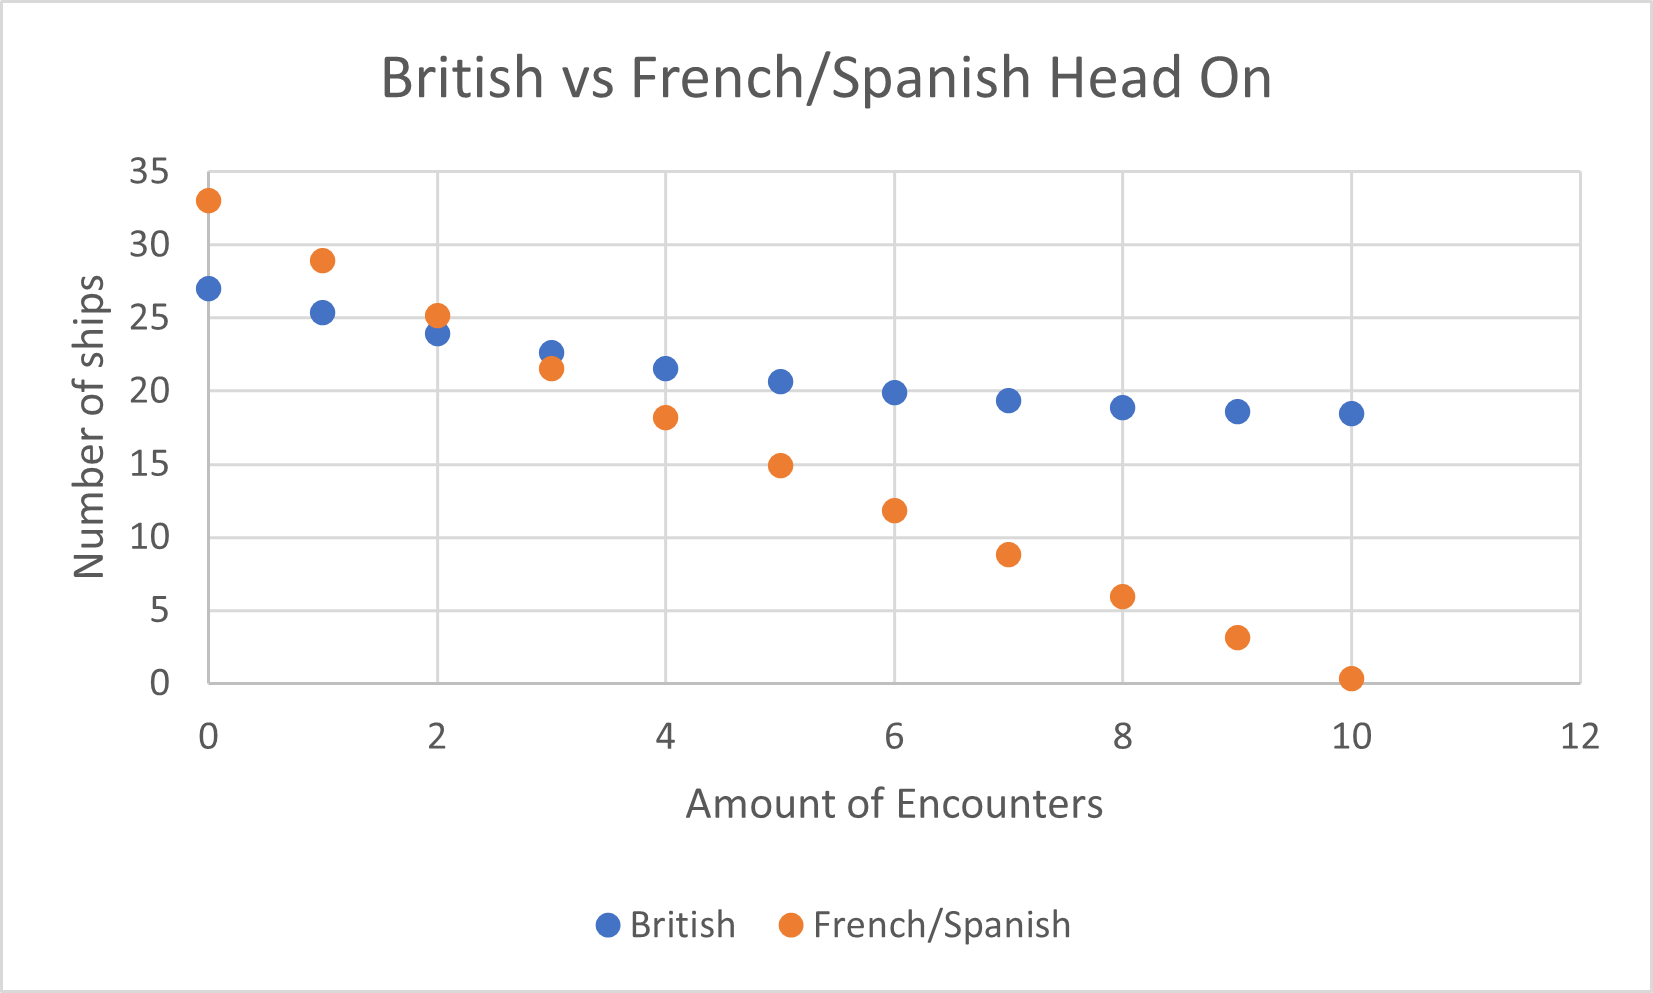
\includegraphics[scale=.7]{1.4 number 3.png}}
      \caption{\label{fig:1} British vs French/Spanish Head On}
    \end{figure}
    \pagebreak
    \item Applying the divide and conquer strategy, we see the British win by an even more 
    extraordinary amount. 
    \begin{figure}[!htb]
      \center{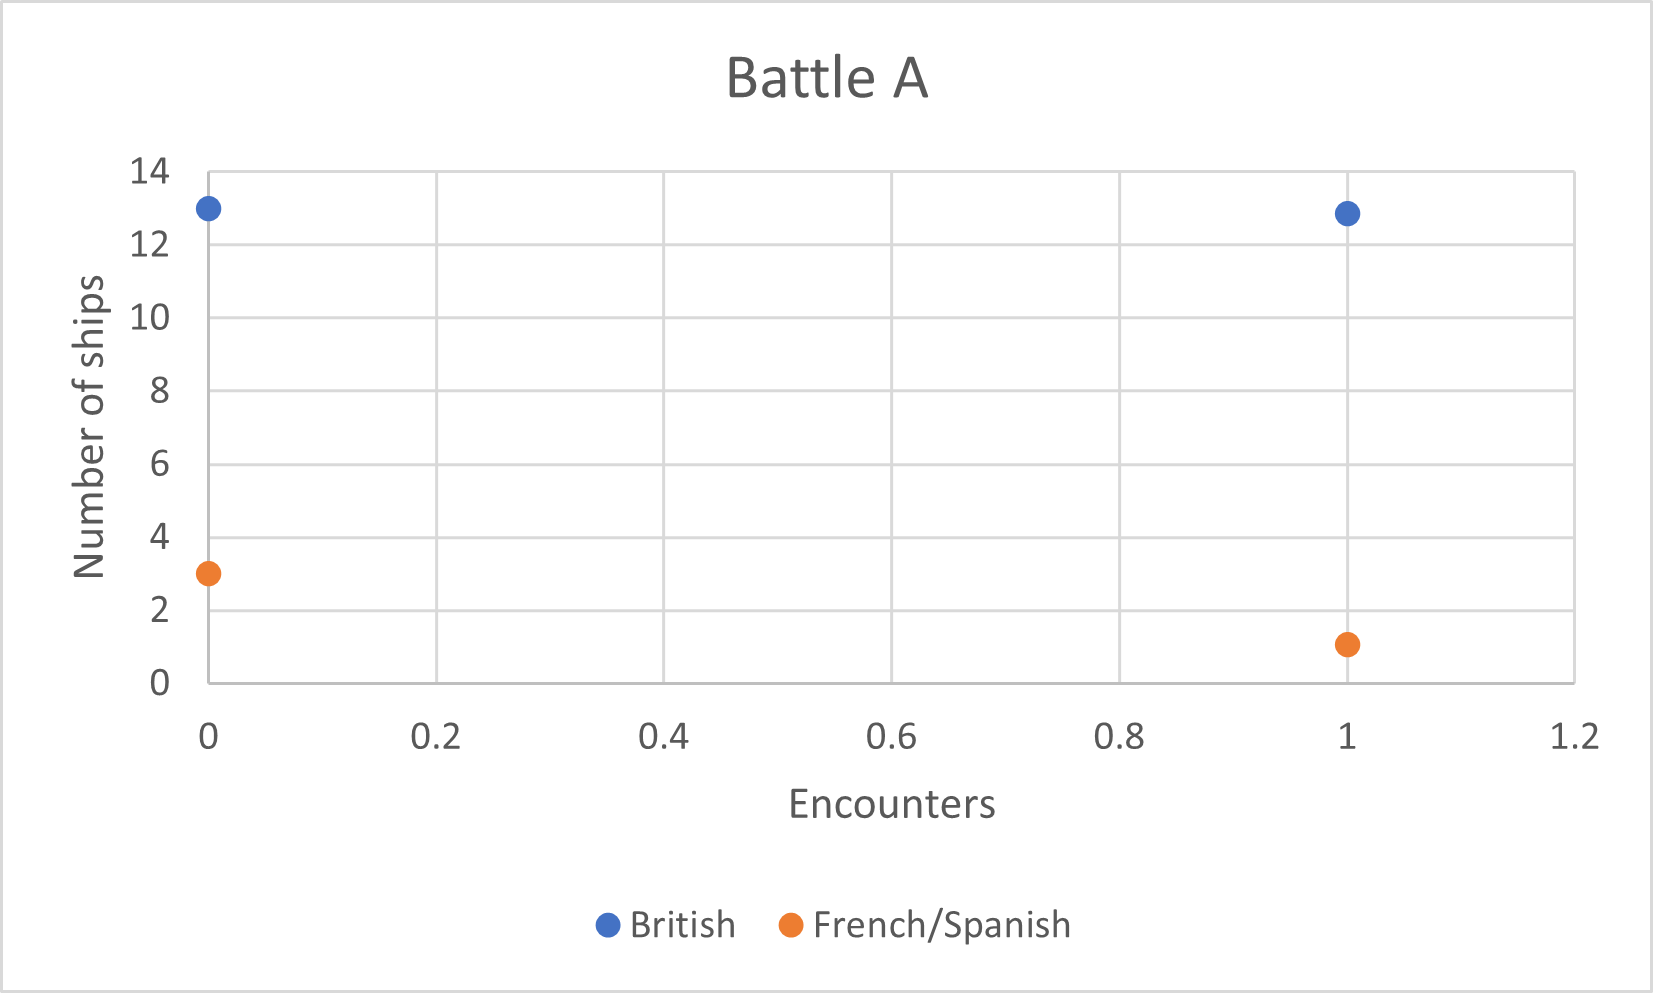
\includegraphics[scale=.7]{Battle A.png}}
      %\caption{\label{fig:2} British vs French/Spanish Head On}
      \center{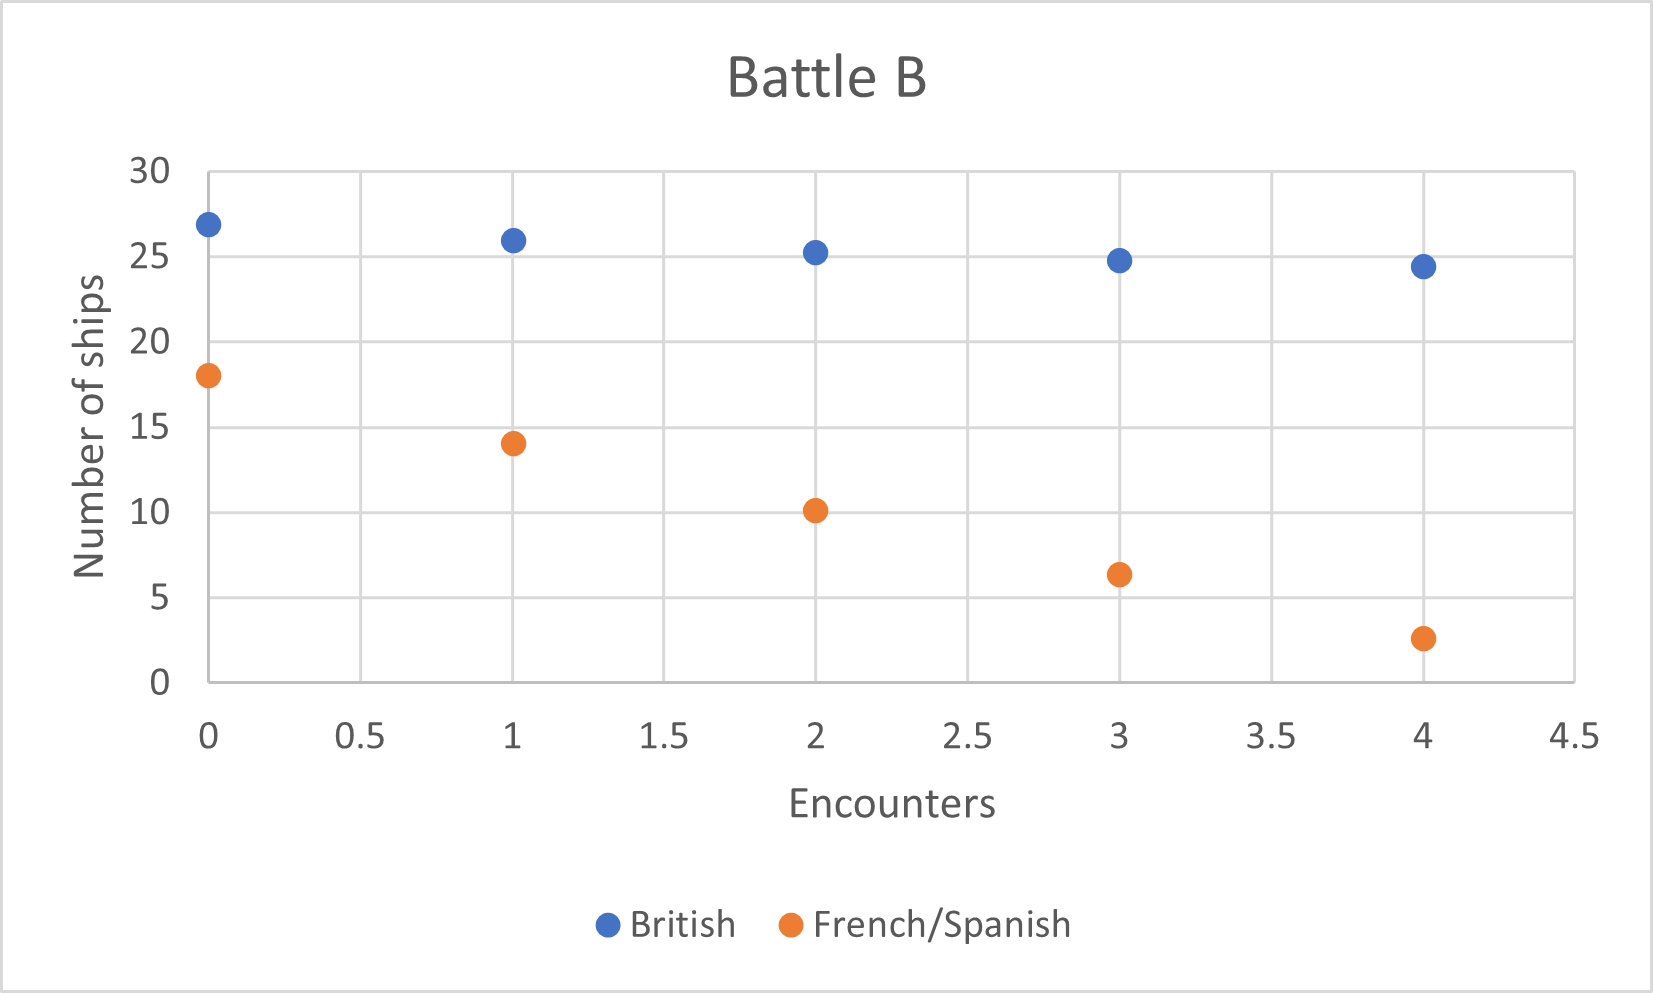
\includegraphics[scale=.7]{Battle B.png}}
      %\caption{\label{fig:2} British vs French/Spanish Head On}
      \center{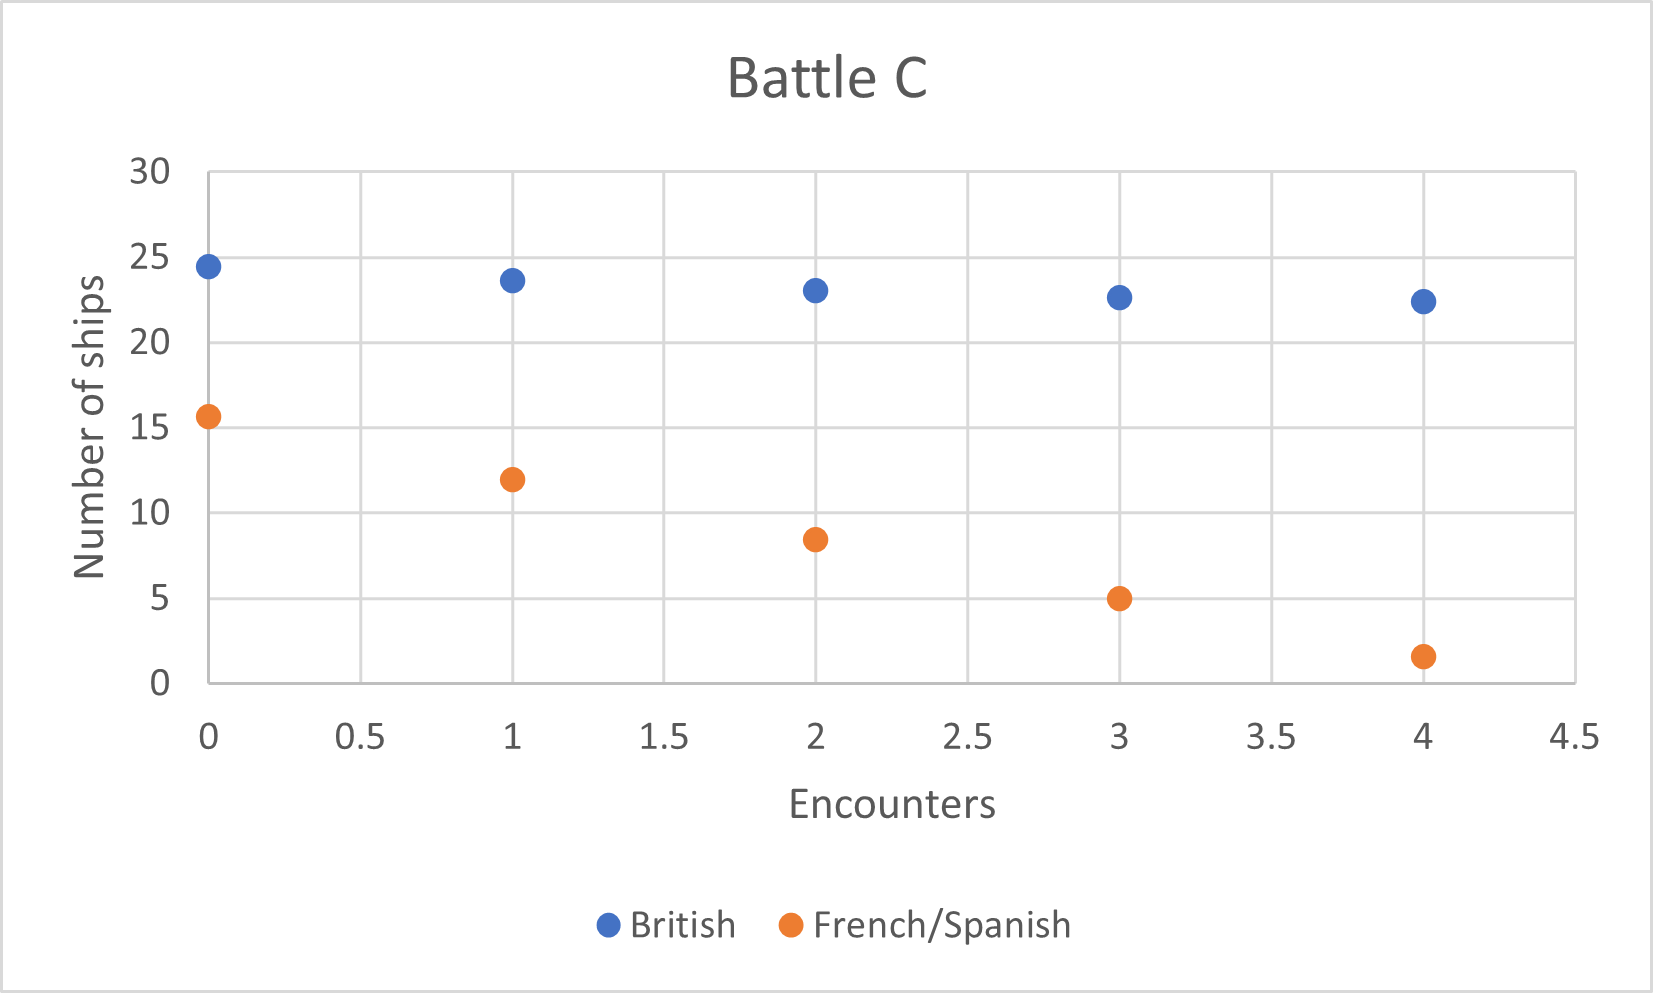
\includegraphics[scale=.7]{Battle C.png}}
      \caption{\label{fig:2} British vs French/Spanish Head On}
    \end{figure}

  \end{enumerate}

\item 1.4) \#4
\begin{enumerate}
  \item The owls in example 3 and the mice in this problem are modelled exactly the same. 
    However, the hawks in example 3 and the owls in this problem are modelled differntly. 
    In example 3, since the coefficient in front of the $H_{n}$ term was greater than 1, 
    the hawk's population would increase if there were no interactions between the owls 
    and the hawks. However, in this problem, the coefficient infront of the $O_{n}$ term
    is less than 1, meaning if there are no interactions between the owls and the mice, 
    the owl population would decrease. The signs in the numbers 1.2, 0.7, .002 indicates 
    these terms will add to their correlating population, while the -0.001 term will 
    subtract from the total population.
  \item The graphs of the owl and mice populations with varying initial conditions
    \begin{figure}[!htb]
      \center{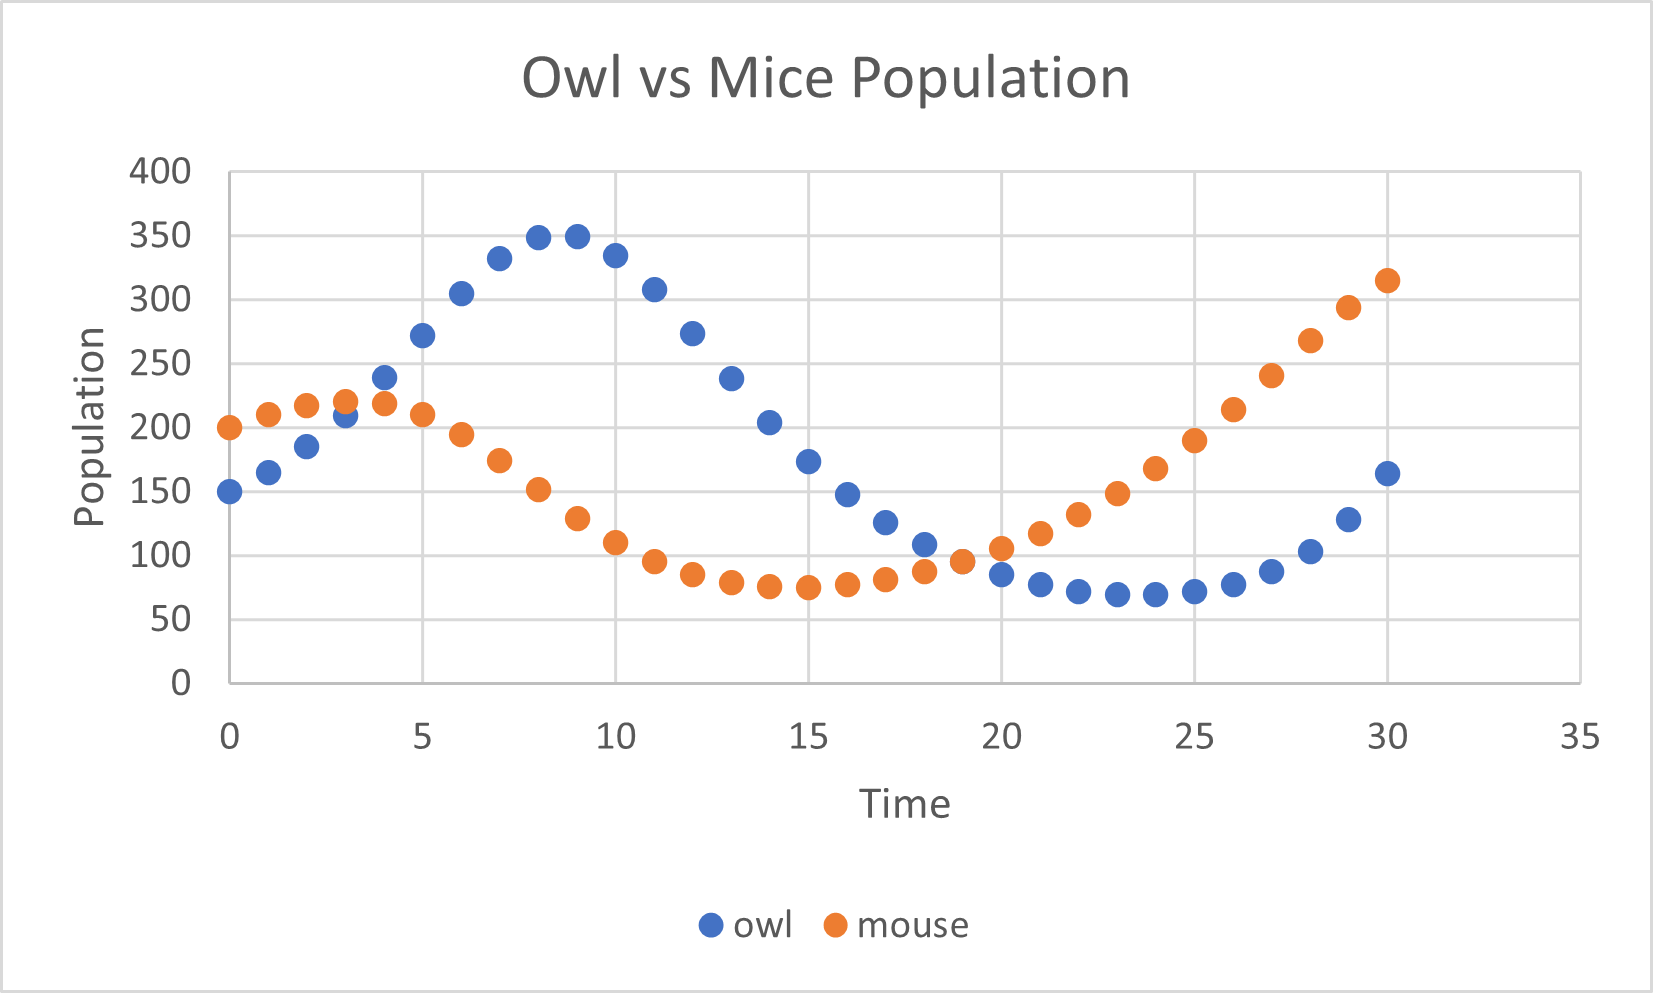
\includegraphics[scale=.65]{150,200.png}}
      \caption{\label{fig:3} Owl vs Mouse Population graphs.}
    \end{figure}
    \begin{figure}[!htb]
      \center{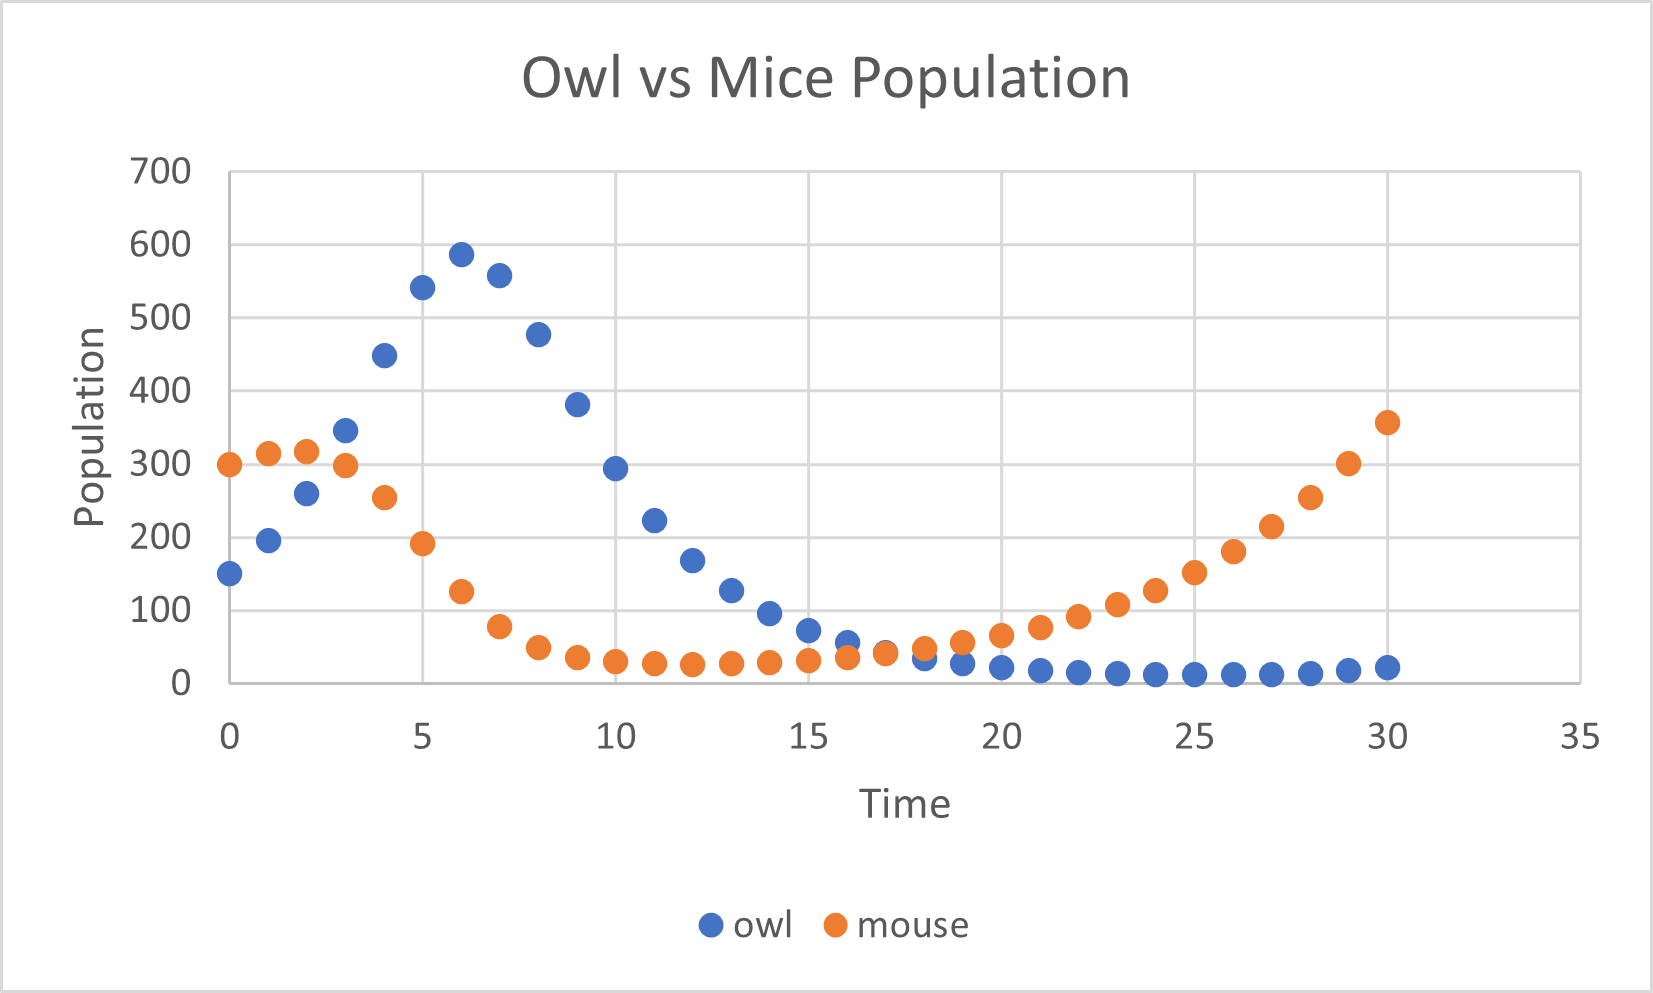
\includegraphics[scale=.65]{150,300.png}}
      \caption{\label{fig:4} Owl vs Mouse Population graphs.}
    \end{figure}
    \begin{figure}[!htb]
      \center{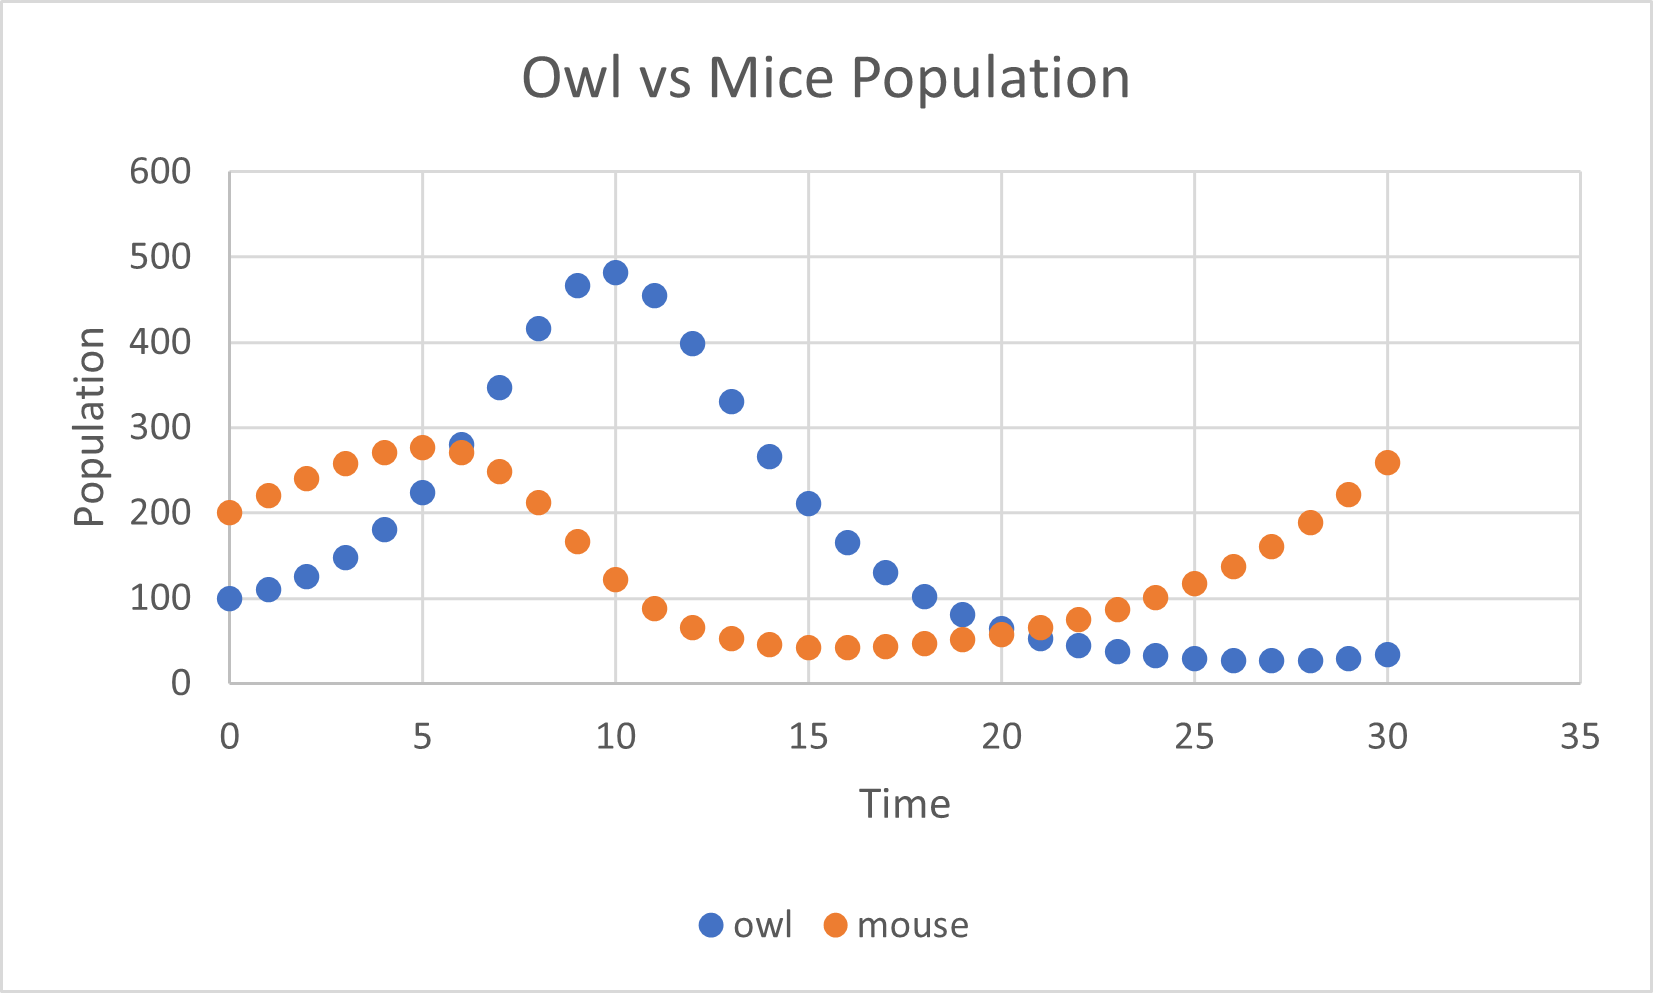
\includegraphics[scale=.65]{100,200.png}}
      \caption{\label{fig:5} Owl vs Mouse Population graphs.}
    \end{figure}
    \begin{figure}[!htb]
      \center{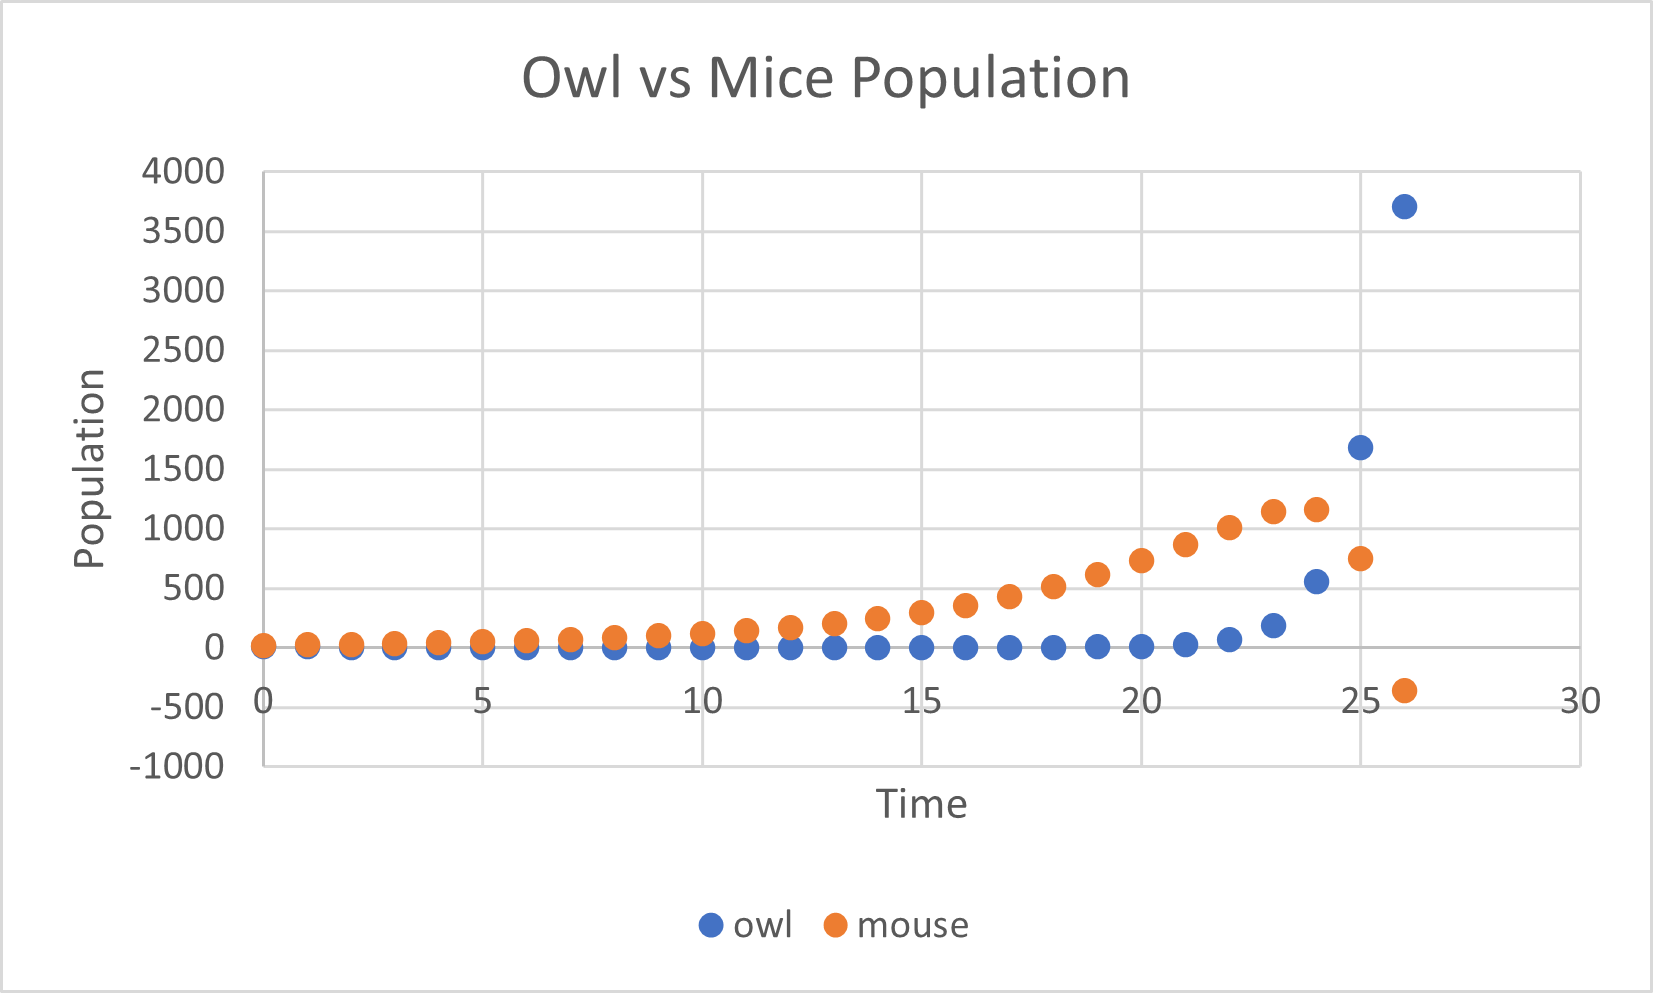
\includegraphics[scale=.65]{10,20.png}}
      \caption{\label{fig:6} Owl vs Mouse Population graphs.}
    \end{figure}
    \pagebreak
  \item Changing around our coefficients, we see this population model is sensitive to 
  changes in the coefficients. By changing our coefficients while keeping our initial 
  values the same, we see the graphs change drastically. 
\end{enumerate}

\item 1.4) \#6
  \begin{enumerate}
    \item Intuitively, the system is saying the price will go up as long as the quantity
    is below 500 and the quantity will go down as long as the price is below 100. Once the 
    price goes above 100, the quantity will start to go up, and once the quantity goes 
    above 500, the price starts to go down. The coefficients represent the rate at which 
    the price and quantity affect each other and the signs show whether the price or quantity
    increase or decrease with this term. 
    \pagebreak
    \item 
    \begin{enumerate}
      \item Case A: These initial values make the second term in both systems disappear, therefore
            this will be an equilibrium solution. 
      \item Case B: 
            \begin{figure}[!htb]
              \center{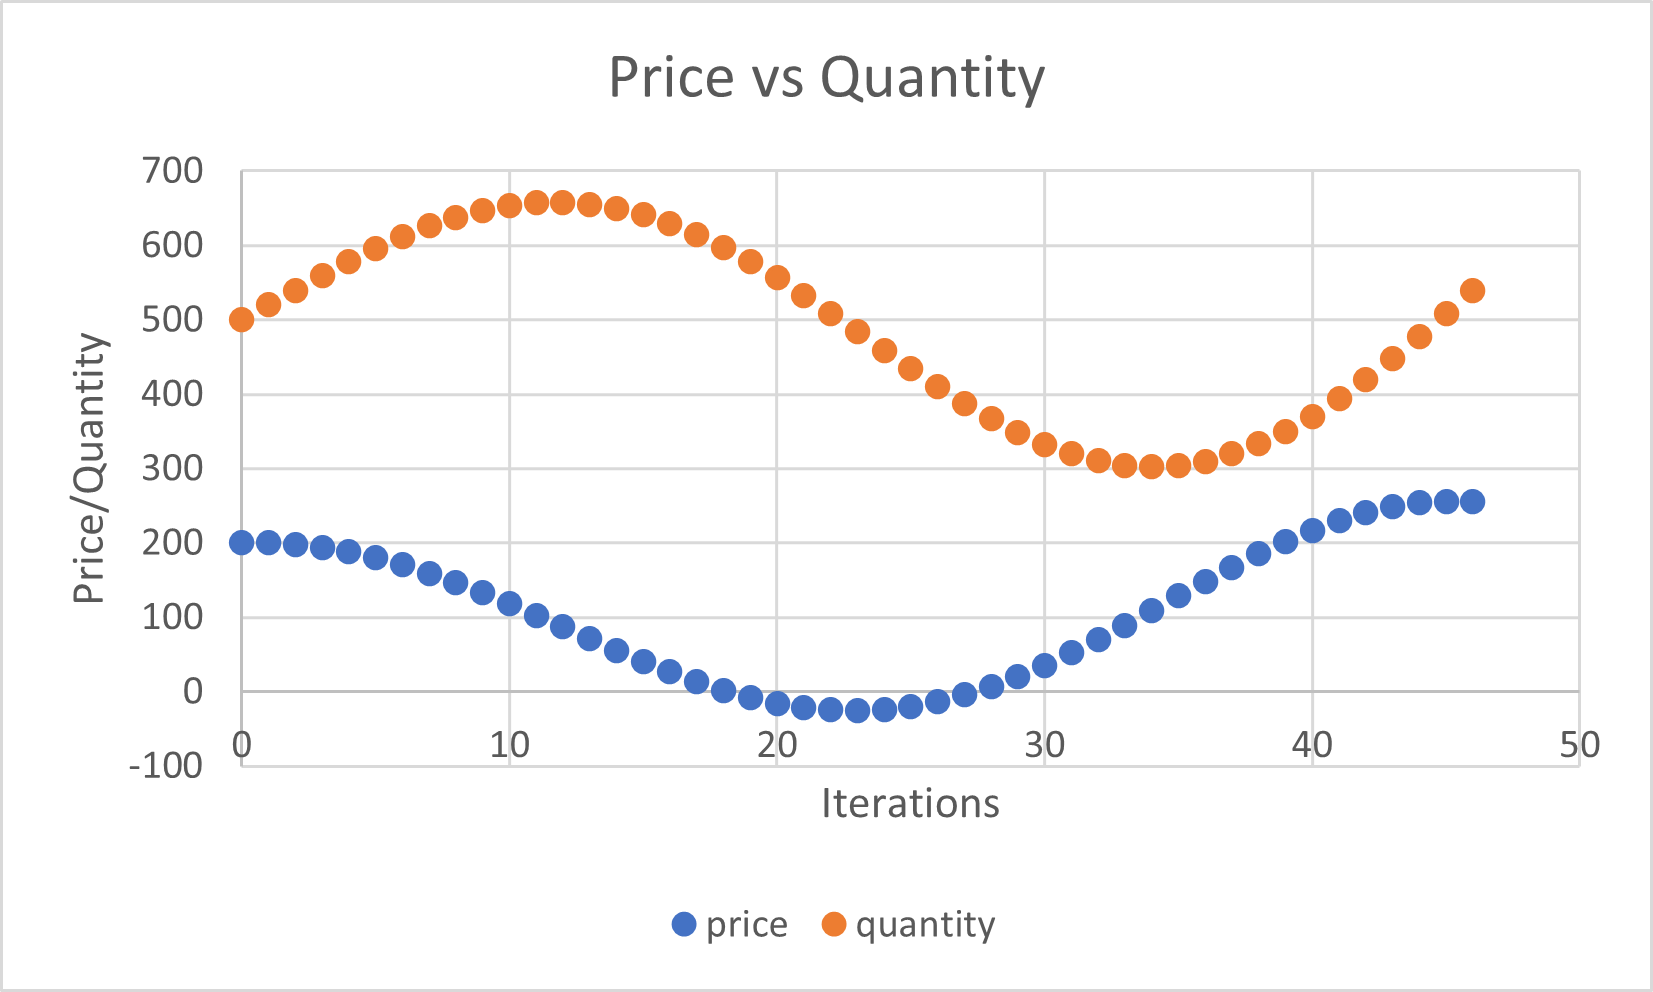
\includegraphics[scale=.6]{200, 500.png}}
              \caption{\label{fig:7} Price vs Quantity}
            \end{figure}
      \item Case C: 
            \begin{figure}[!htb]
              \center{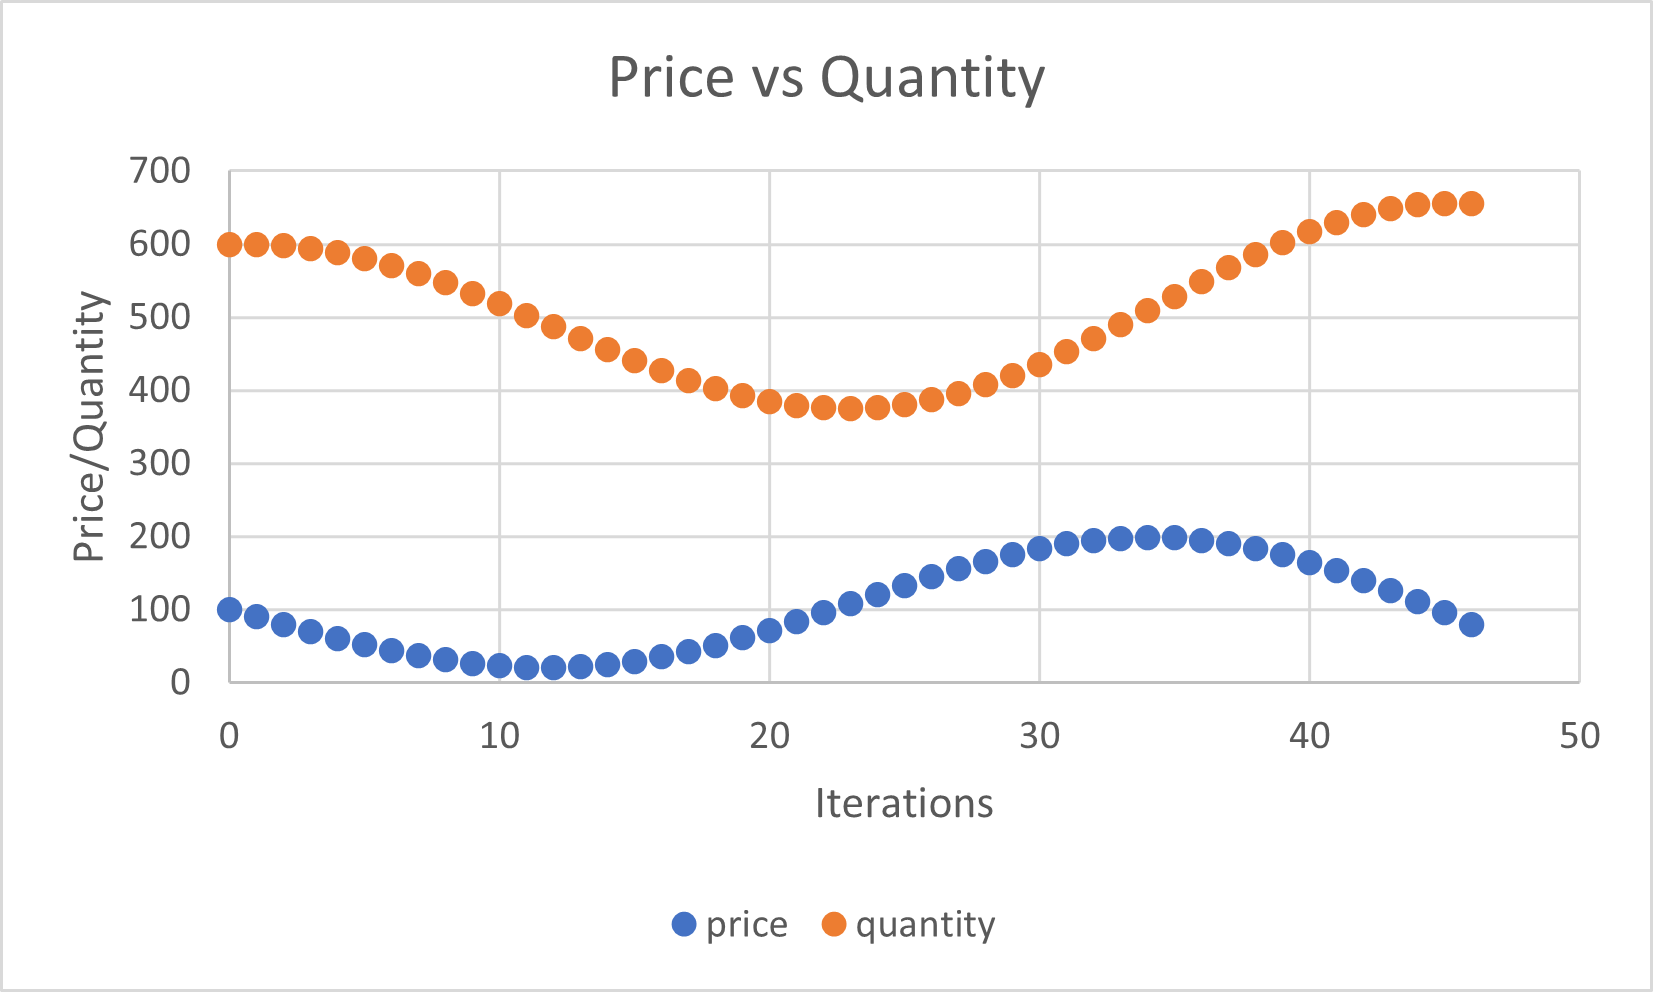
\includegraphics[scale=.6]{100, 600.png}}
              \caption{\label{fig:8} Price vs Quantity}
            \end{figure}
      \item Case D: 
            \begin{figure}[!htb]
              \center{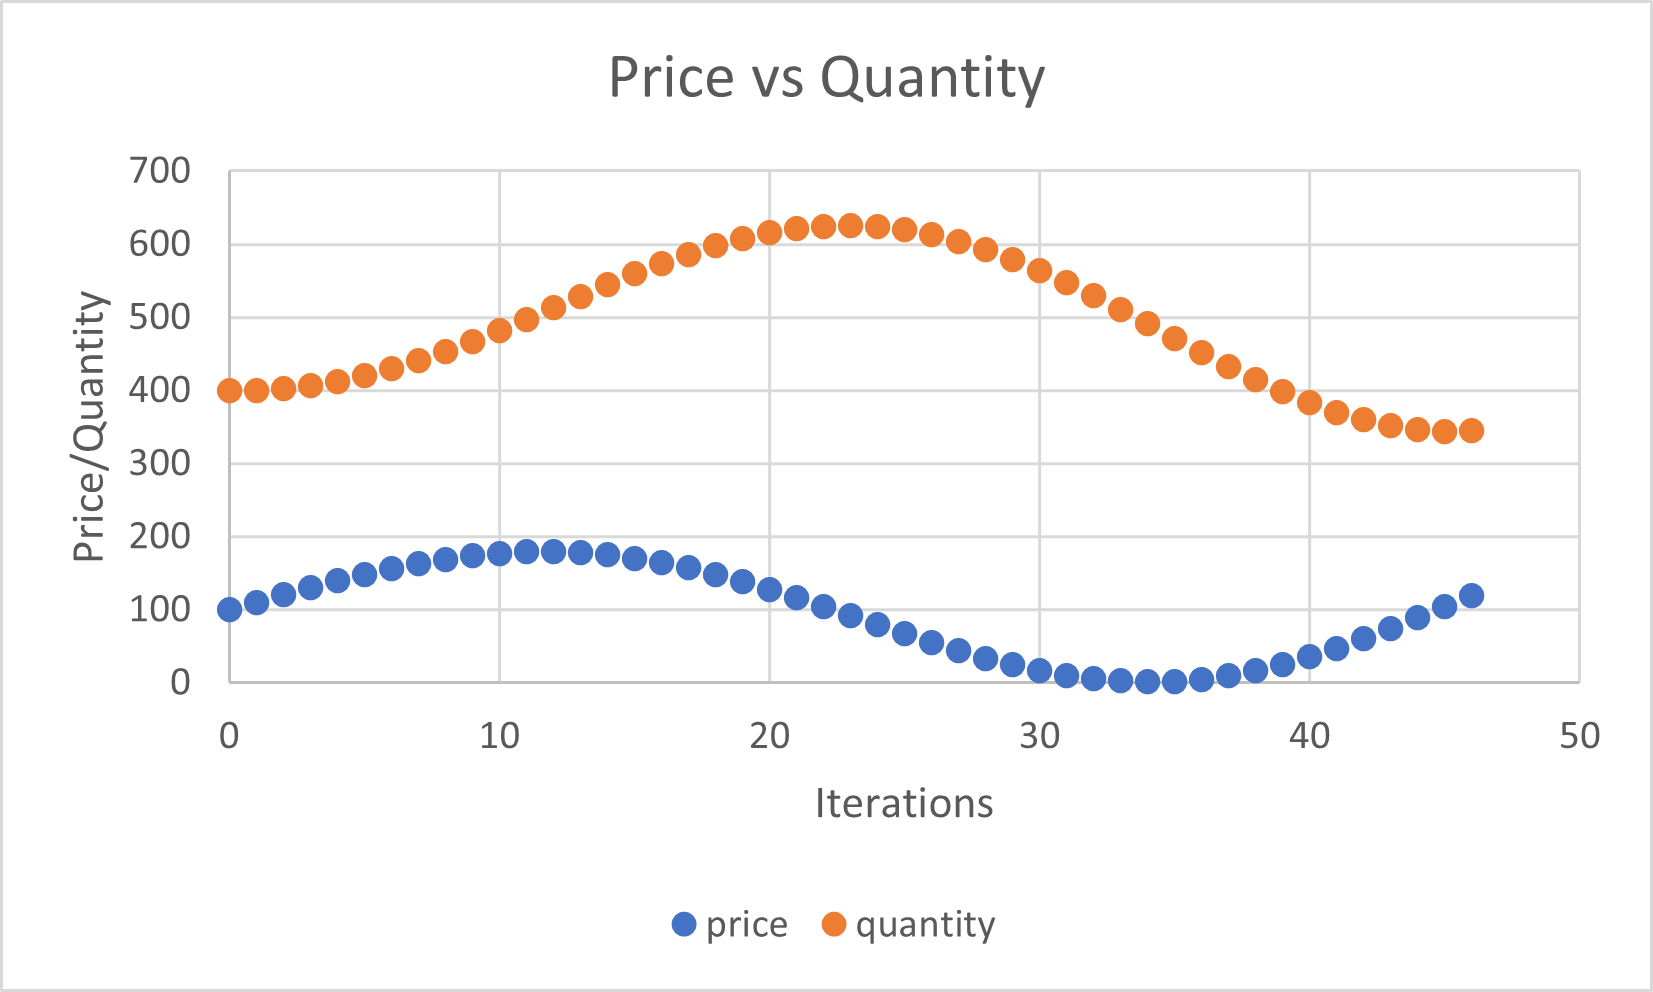
\includegraphics[scale=.6]{100, 400.png}}
              \caption{\label{fig:9} Price vs Quantity}
            \end{figure}
    \end{enumerate}
    We see from Case B, C and D, we see that the price and the quantity of the product
    oscillate, with the price going below zero at certain points in the plot. The graphs
    also seem to oscillate around the same point: 500 for quantity, and 100 for price. 
  \end{enumerate}
  
\item 1.4) \#10 (SIR Problem)
Our original model: 
\center{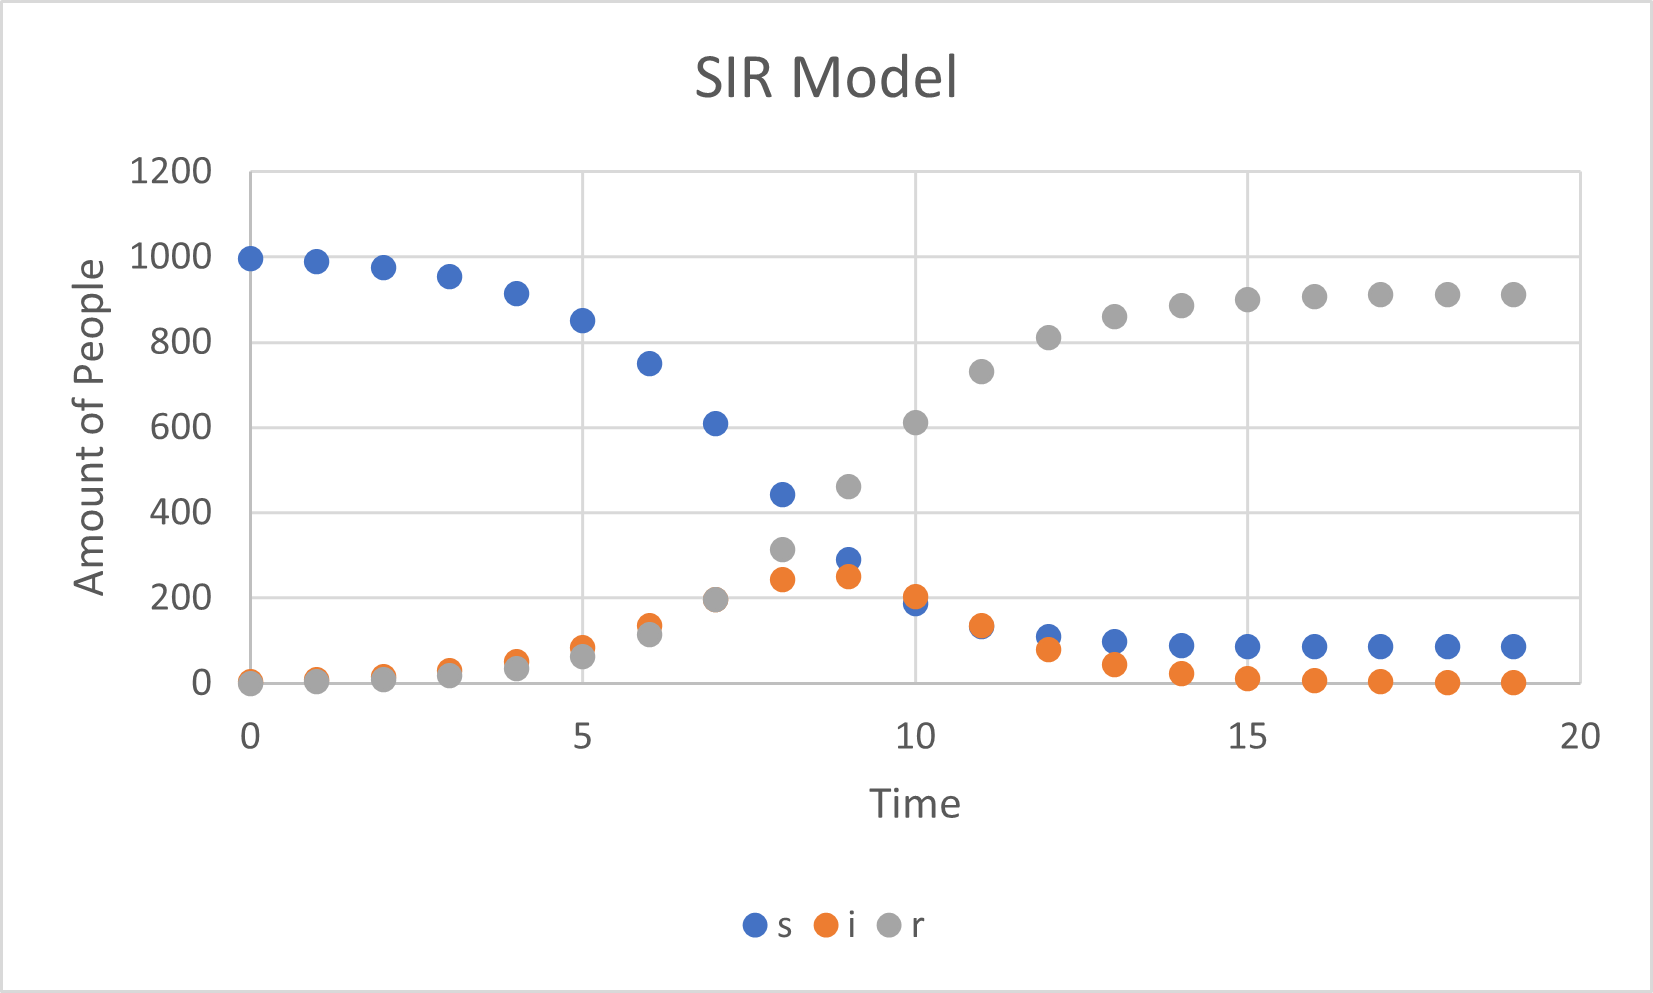
\includegraphics[scale=.7]{SIRoriginal.png}}
\begin{enumerate}
  \item With the initial conditions changed to $I_{0} = 5, I_{1} = 15$
  \begin{eqnarray*}
    I_{0} = 5, I_{1} = I_{0}-.6I_{0}+aI_{0}S_{0}\\
    I_{1} = 5 - .6(5) + a(5)(995) = 15\\
    a = \frac{15-5+3}{5(995)}\\
    a = 0.002613
  \end{eqnarray*}
  Therefore, our new model is: 
  \begin{eqnarray*}
    S_{n+1} = S_{n} - 0.002613S_{n}I_{n}\\
    I_{n+1} = I_{n} - .6I_{n} + 0.002613S_{n}I_{n}\\
    R_{n+1} = R_{n} + .6I_{n} \\
    I_{0} = 5, S_{0} = 995, R_{0} = 0
  \end{eqnarray*}\\
  with the new model, our plot looks like: 
  \begin{figure}[!htb]
    \center{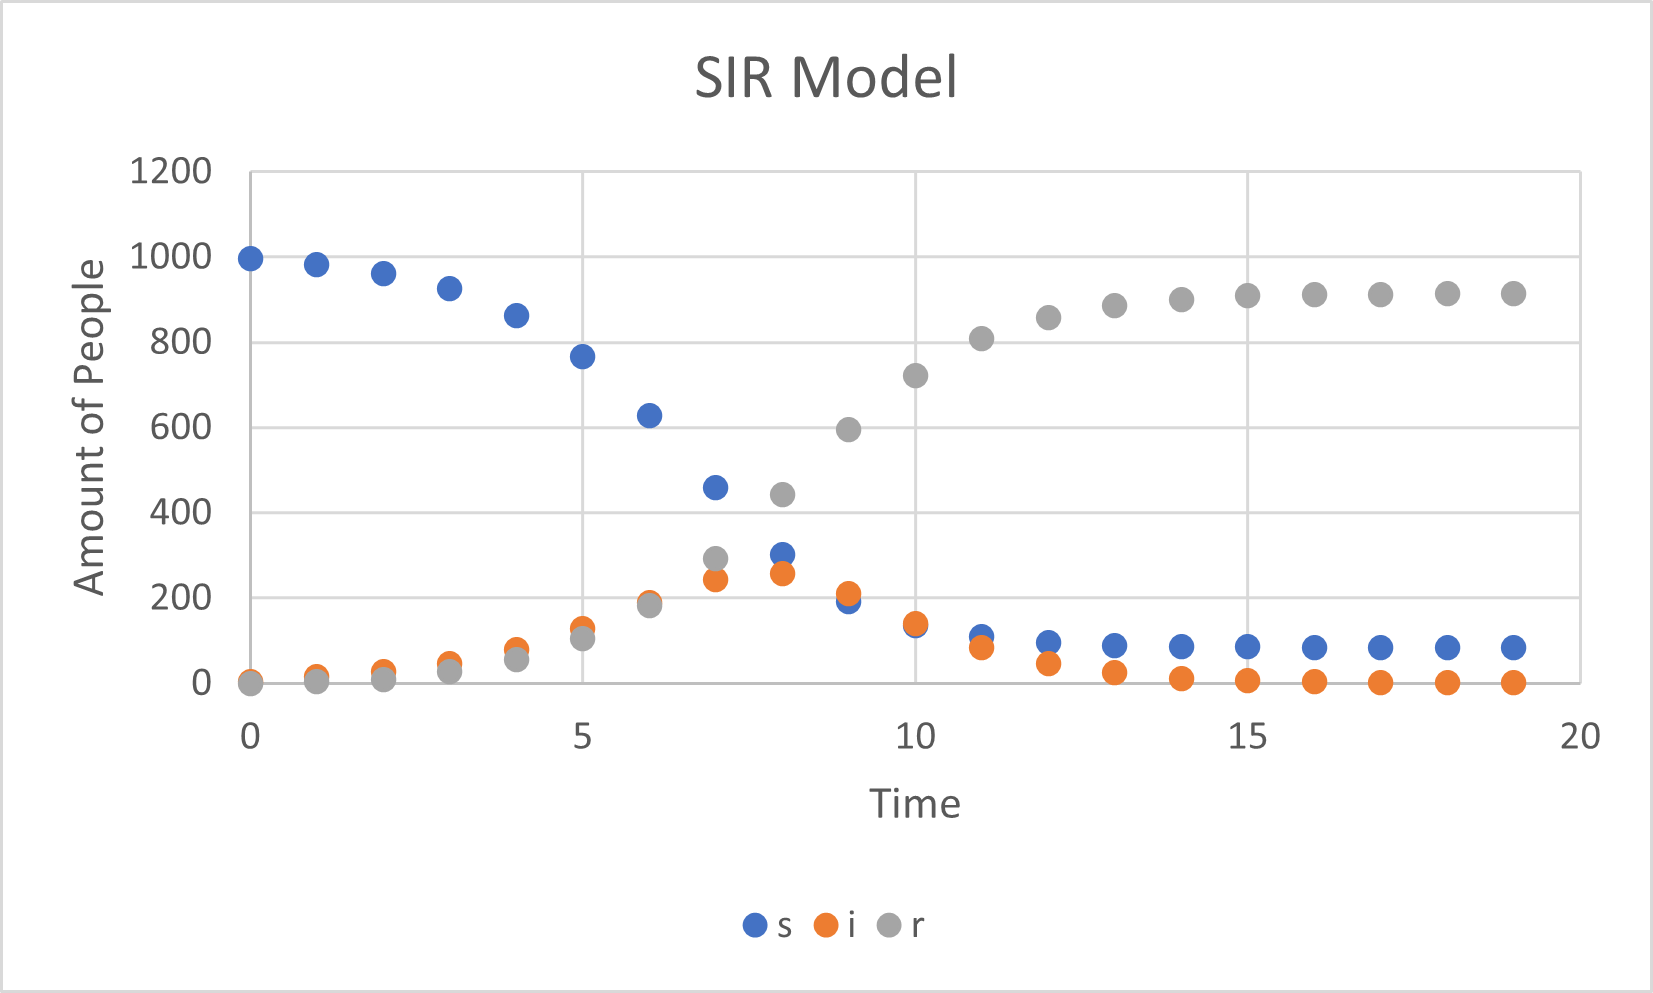
\includegraphics[scale=.7]{SIRa.png}}
    \caption{\label{fig:10} SIR model with $I_{0} = 5, I_{1} = 15$}
  \end{figure}
  where the point of intersection between the S, I, and R seem to intersect a bit 
  earlier, but otherwise seem to be quite similar to our original. 

  \item With the initial conditions changed so the flu lasts 1 week: 
  \begin{eqnarray*}
    S_{n+1} = S_{n} - 0.001407S_{n}I_{n}\\
    I_{n+1} = I_{n} - 1I_{n} + 0.001407S_{n}I_{n}\\
    R_{n+1} = R_{n} + 1I_{n} \\
    I_{0} = 5, S_{0} = 995, R_{0} = 0
  \end{eqnarray*}
  with the new model, our plot looks like: 
  \begin{figure}[!htb]
    \center{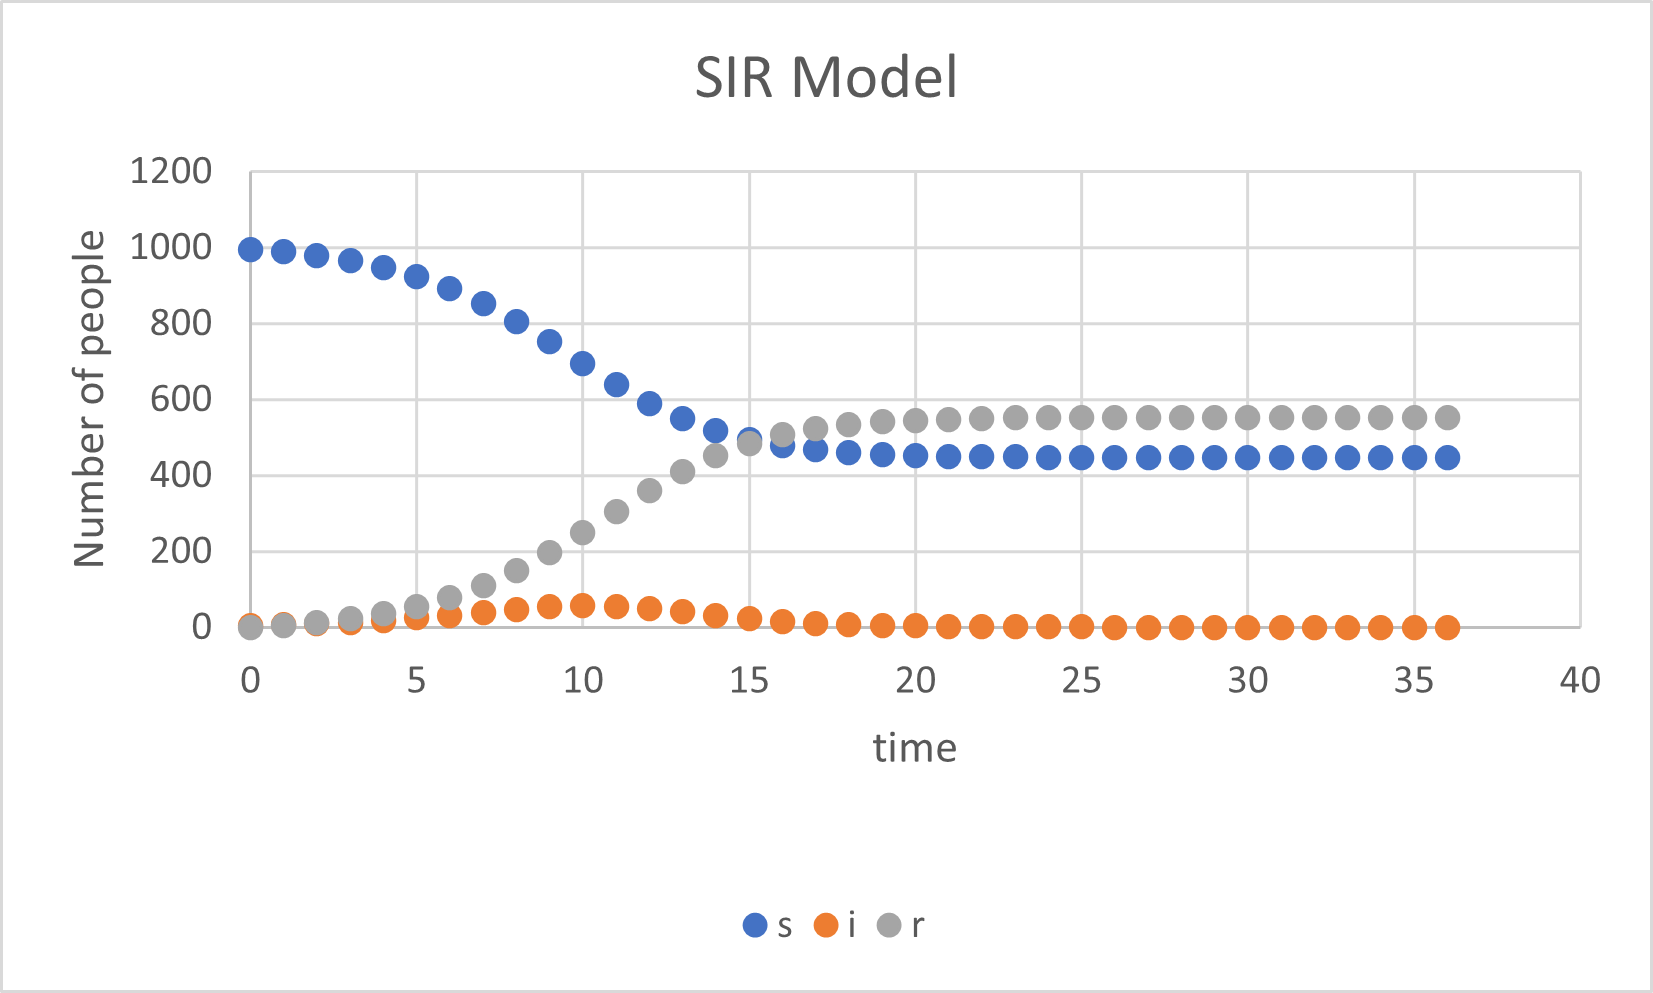
\includegraphics[scale=.7]{SIRb.png}}
    \caption{\label{fig:11} SIR model with flu lasts 1 week}
  \end{figure}\\
  We see if the flu only lasts one week, the amount of people who even get the flu is 
  quite low, and since the amount of infected people is quite low, there are less chances
  to get the flu, resulting in people recovering faster than people getting the flu. Then, 
  even though there are many people still susceptible, there are no people to catch the 
  flu from, resulting in zero infected people within 20 weeks. 

  \item With the initial conditions changed so the flu lasts 4 weeks: 
  \begin{eqnarray*}
    S_{n+1} = S_{n} - 0.001407S_{n}I_{n}\\
    I_{n+1} = I_{n} - .25I_{n} + 0.001407S_{n}I_{n}\\
    R_{n+1} = R_{n} + .25I_{n} \\
    I_{0} = 5, S_{0} = 995, R_{0} = 0
  \end{eqnarray*}
  with the new model, our plot looks like: 
  \begin{figure}[!htb]
    \center{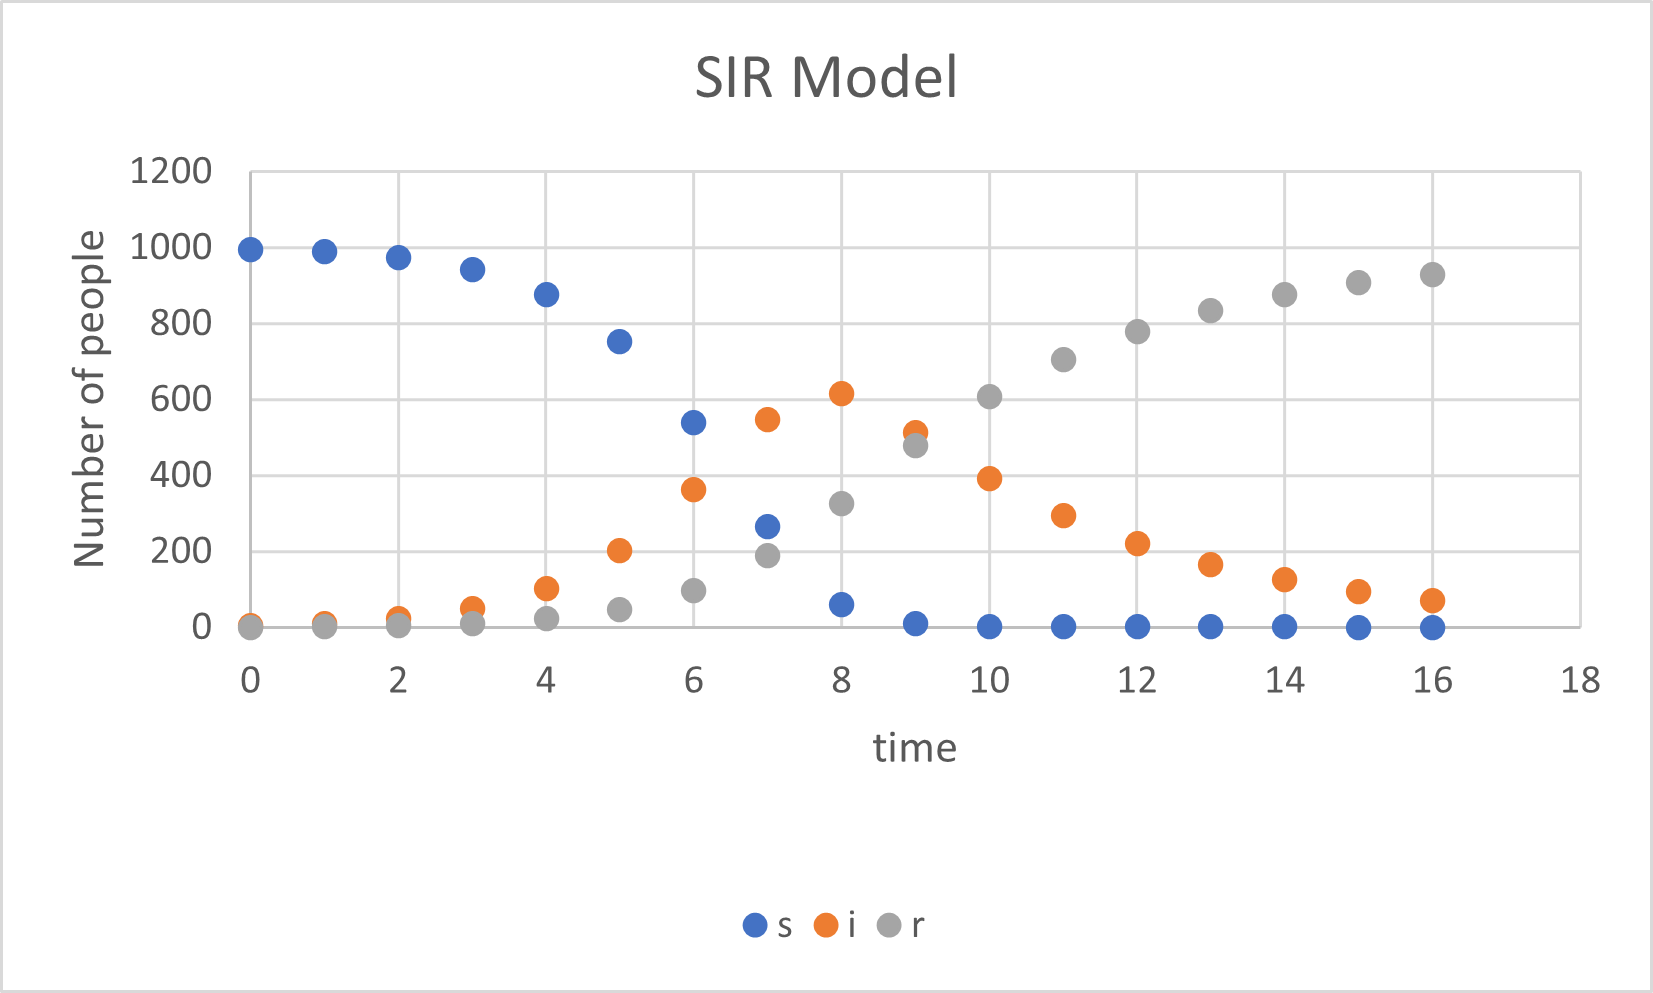
\includegraphics[scale=.7]{SIRc.png}}
    \caption{\label{fig:12} SIR model with flu lasts 4 weeks}
  \end{figure}\\
\pagebreak
  Changing the flu to last 4 weeks, we see the number of infected people spikes very high
  compared to our original model. The number of susceptible people also goes down very quickly, 
  while the removed seems to be somewhat slower than our original model. We see the flu seems to 
  be a bit more dramatic when it lasts 4 weeks instead of our original 5/3. 

  \item With 4000 students in the dorm, 5 infected and 30 more the next week: 
  \begin{eqnarray*}
    I_{0} = 5, I_{1} = I_{0}-.6I_{0}+aI_{0}S_{0}\\
    I_{1} = 5 - .6(5) + a(5)(3995) = 30\\
    a = \frac{30-5+3}{5(3995)}\\
    a = 0.001402
  \end{eqnarray*}
  Therefore, our new model is: 
  \begin{eqnarray*}
    S_{n+1} = S_{n} - 0.001402S_{n}I_{n}\\
    I_{n+1} = I_{n} - .6I_{n} + 0.001402S_{n}I_{n}\\
    R_{n+1} = R_{n} + .6I_{n} \\
    I_{0} = 5, S_{0} = 3995, R_{0} = 0
  \end{eqnarray*}
  with the new model, our plot looks like: 
  \begin{figure}[!htb]
    \center{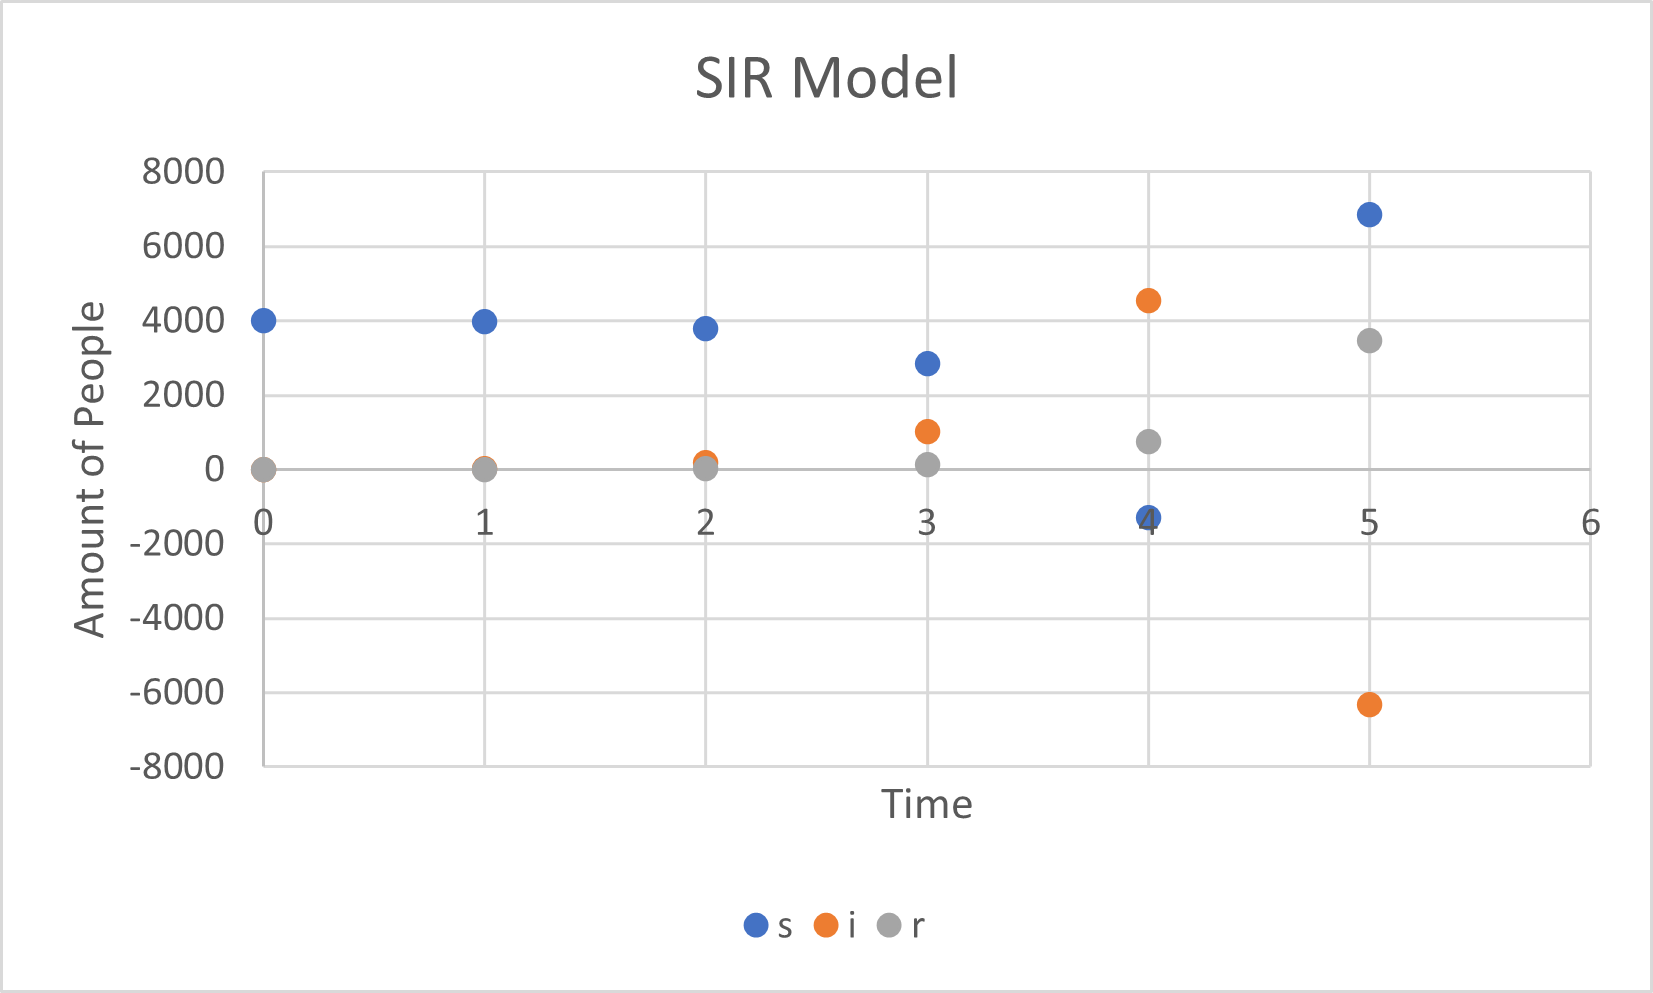
\includegraphics[scale=.7]{SIRdpng.png}}
    \caption{\label{fig:13} SIR model with $I_{0} = 5, S_{0} = 3995$}
  \end{figure}\\
\pagebreak
  We see with the amount of students increased, there are more chances for interactions, 
  even though the infection rate is quite similar. Because of this, we see the virus spreads
  much faster than before and weeks seem to be somewhat of an inadequate measure of time 
  to model with this many students in dorms, for example, by week 4, the number of susceptible 
  students is negative, meaning sometime between weeks 3 and 4, everyone susceptible should have 
  been either infected or removed, but our model overshoots and becomes negative. 
\end{enumerate}
\pagebreak
\item Write a python program that will sum the first 100 integers.
  \emph{Solution.} \\
  \begin{figure}[!htb]
    \center{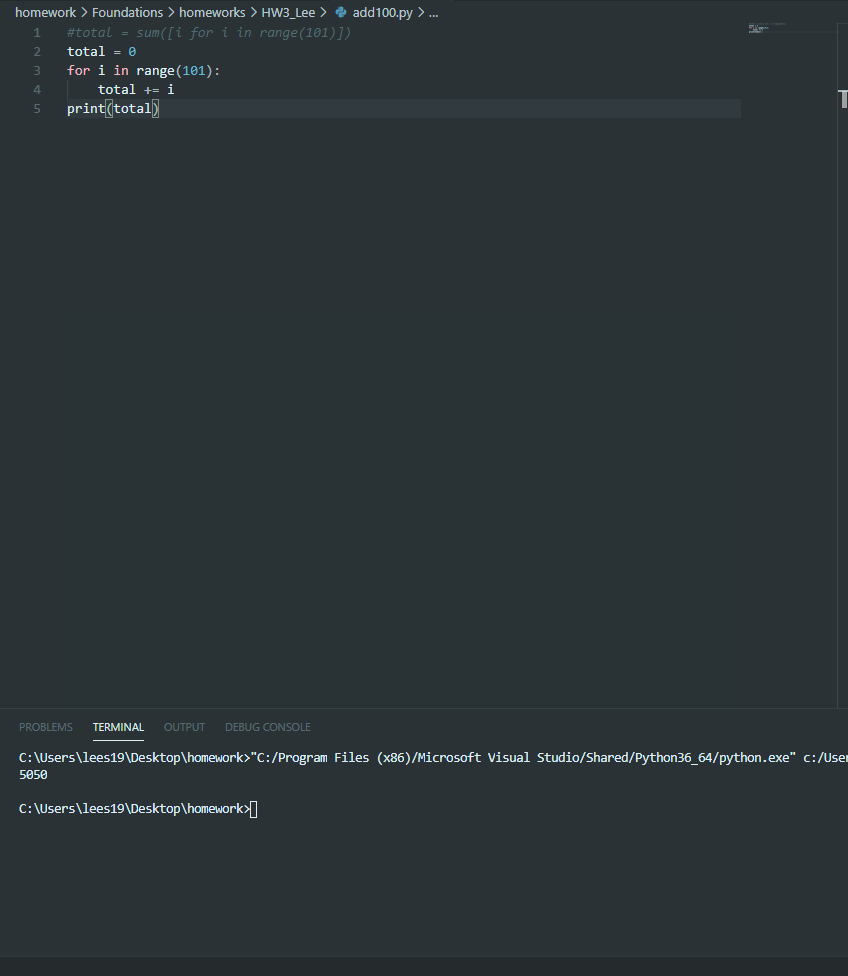
\includegraphics[scale=.7]{python.png}}
    \caption{\label{fig:} }
  \end{figure}

\end{enumerate}


\end{document}